\documentclass{standalone}
\usepackage{tikz}
\begin{document}
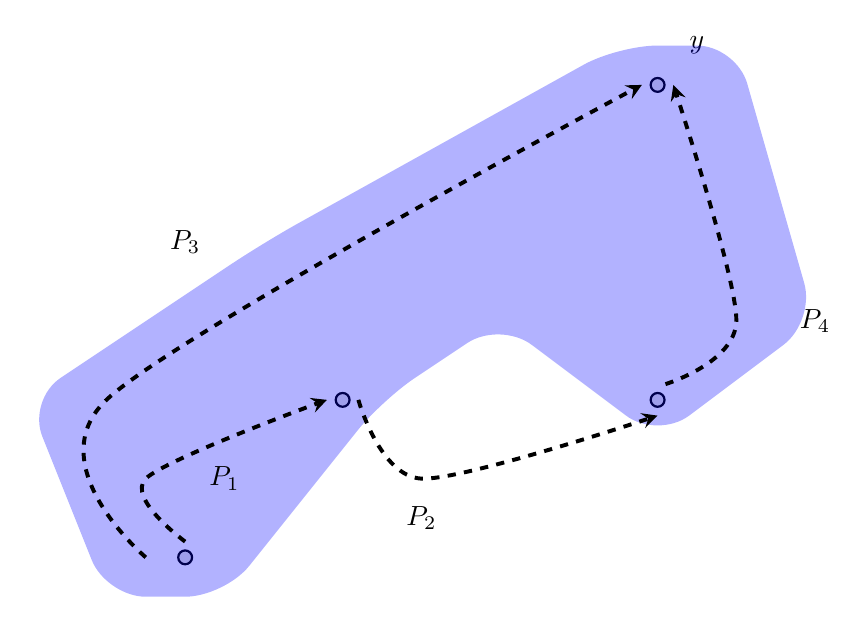
\begin{tikzpicture}
    \coordinate (y) at (2,2);
    \node at ([shift={(0.5,0.5)}]y) {$y$};
    \coordinate (v) at (-2,-2);
    \coordinate (w) at (2,-2);
    \coordinate (ti) at (-4,-4);
    \node[draw,circle,fill=gray!20,thick,inner sep=1pt,minimum size=5pt] (CircleNode) at (v)  {};
    \node[draw,circle,fill=gray!20,thick,inner sep=1pt,minimum size=5pt] (CircleNode) at (w)  {};
    \node[draw,circle,fill=gray!20,thick,inner sep=1pt,minimum size=5pt] (CircleNode) at (y)  {};
    \node[draw,circle,fill=gray!20,thick,inner sep=1pt,minimum size=5pt] (CircleNode) at (ti)  {};

    \draw [draw=none,rounded corners = 5mm,fill=blue,fill opacity=0.3] ([shift={(-0.5,0.5)}]y)--([shift={(-5,-2)}]y)--([shift={(-2,2)}]ti)--([shift={(-1,-0.5)}]ti)--([shift={(0.5,-0.5)}]ti)--([shift={(0.5,0)}]v)--([shift={(2,1)}]v)--([shift={(0,-0.5)}]w)--([shift={(2,1)}]w)--([shift={(1,0.5)}]y)--cycle; 

    \draw[line width=0.5mm,dashed,-stealth] plot[smooth] coordinates {([shift={(-0.5,0)}]ti)([shift={(-1,2)}]ti)([shift={(-0.2,0)}]y)};
    \node at ([shift={(0,4)}]ti) {$P_3$};
    \draw[line width=0.5mm,dashed,-stealth] plot[smooth] coordinates {([shift={(0,0.2)}]ti)([shift={(-0.5,1)}]ti)([shift={(-0.2,0)}]v)};
    \node at (-3.5,-3) {$P_1$};
    \draw[line width=0.5mm,dashed,-stealth] plot[smooth] coordinates {([shift={(0.2,0)}]v)([shift={(1,-1)}]v)([shift={(0,-0.2)}]w)};
    \node at ([shift={(1,-1.5)}]v){$P_2$};
    \draw[line width=0.5mm,dashed,-stealth] plot[smooth] coordinates {([shift={(0.1,0.2)}]w)([shift={(1,1)}]w)([shift={(0.2,0)}]y)};
    \node at ([shift={(2,1)}]w){$P_4$};
\end{tikzpicture}
\end{document}